\section{Clock time and calendar date}
\label{sec-clock-calendar}

\textbf{Created by:} Arkopaul Sarkar \\
\textbf{Modified by:} Arkopaul Sarkar \\

\subsection*{Scenario Objective}

This scenario illustrates how to associate clock time and calendar dates with instances of time. While the ability to store clock time and calendar dates allows users to perform various quantitative analyses on the processes and their durations, the wide variety of clock and calendar systems presents challenges in accurately representing dates and times in the correct format. We include use cases depicting both basic and advanced methods for representing date and time values of temporal instances.


\subsection*{General Pattern Description}

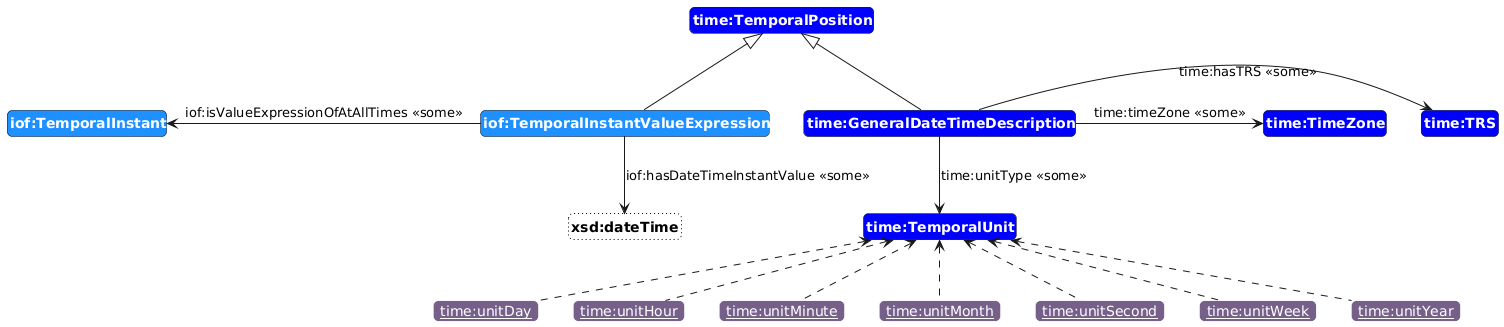
\includegraphics[scale=0.28]{scenarios/clock-time-calendar-date/images/general-clock-calendar.png}

the calendar and clock time for a specific temporal instant can be expressed by associating different instances of the information class \texttt{TemporalInstantValueExpression} or OWL-Time class \texttt{time:General\\DateTimeDescription} as both are subclass of \texttt{time:TemporalPosition} (\texttt{core:TemporalInstantValue\\Expression} is mapped as subclass of \texttt{time:TemporalPosition}.  

\subsubsection*{Use Case: Launch of first iPhone} 
The original iPhone was first launched on June 29, 2007 during the Macworld Conference \& Expo in San Francisco, California. 

The date and time of the launch are captured in 1) XSD dateTime format, 2) in a specific time zone, and 3) using a custom date and time format. The process \texttt{launch-of-iphone} is not detailed further except the temporal interval it occupies. This instance of temporal interval is then connected to its first temporal instant, for which the calendar date and clock time are assigned.   

\subsubsection*{Use-Case Pattern Description}

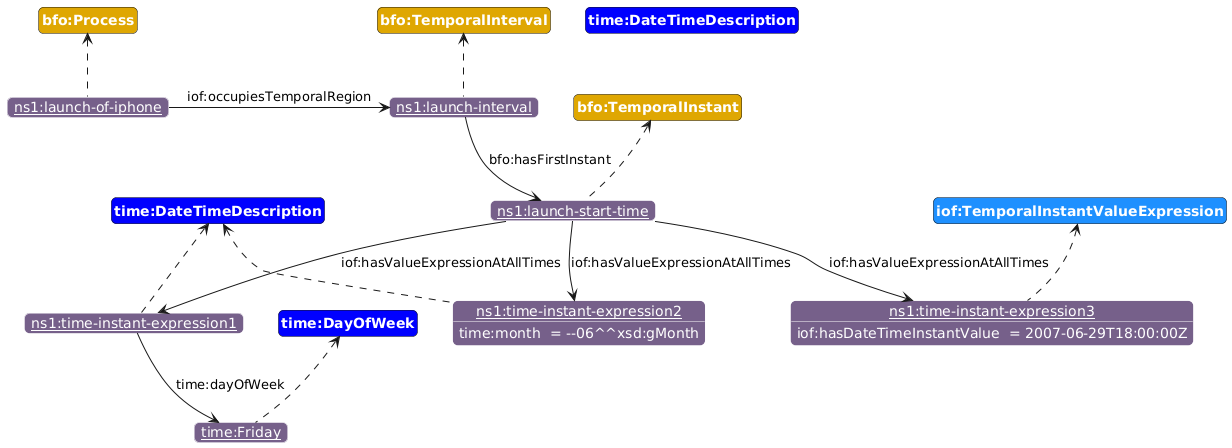
\includegraphics[scale=0.35]{scenarios/clock-time-calendar-date/images/uc1-dow-mn.png}

The launch date and time are expressed in three different ways.  

\texttt{hasDateTimeInstantValue} can associate the date and time value in \texttt{xsd:dateTime} format. If the date and time values can be expressed in XSD format, this pattern does not require any reference to OWL Time ontology. Also, \texttt{xsd:dateTime} format already has provision for mentioning time zone (e.g., 2007-06-29T18:00:00-05:00 for a UTC-5 timezone). However, as XSD:dateTime datatype is the range of \texttt{hasDateTimeInstantValue}, no other XSD type or a different format can be expressed using this pattern. 

\paragraph{Other components of a clock time \\}

In the above pattern, the launch date and time of the iPhone in New York are expressed as `day of the week' using \texttt{time:dayOfWeek} (OWL Time ontology provides the days of a week as instances of type \texttt{time:DayOfWeek})  and `month', using \texttt{time:month} data property \texttt{xsd:gMonth} which links to an indexical value based on the order of months in the calendar of type \texttt{xsd:gMonth} \footnote{\url{https://www.w3.org/TR/xmlschema11-2/\#gMonth}}.
Various combinations of data properties of \texttt{GeneralisedDateTimeDescription}, e.g.,  year, month, day, hour, minute, and second, can be used to express a clock time or calendar date, e.g., only date value in year, month and day. The corresponding time zone can be mentioned by linking an instance of \texttt{TimeZone} \footnote{For detailed guidance about working with time zones, see \url{http://www.w3.org/TR/timezone/} .}, using \texttt{time:timeZone} property.       

\paragraph{Using custom clock time format \\}

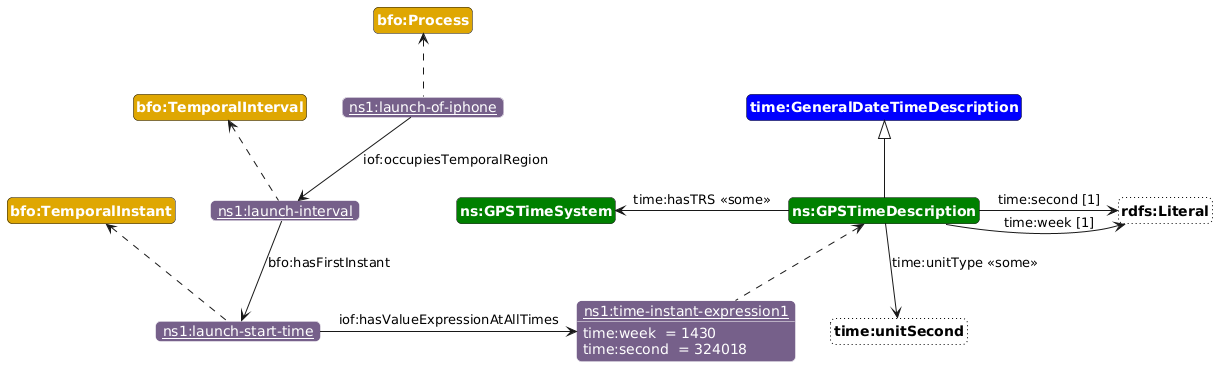
\includegraphics[scale=0.35]{scenarios/clock-time-calendar-date/images/uc1-custom.png}

In the above pattern the launch date is expressed in `GPS time'. As GPS time is the number of seconds since an epoch in 1980, encoded as the number of weeks and seconds into the week, the new class  \texttt{GPSTimeDescription}, extended from \texttt{time:DateTimeDescription}, should contain values for data properties \texttt{time:second} and \texttt{time:week}. The example does not provide details of \texttt{GPSTimeSystem}, which is a \texttt{time:TemporalReferenceSystem}, and may refer to a suitable description of `GPS time', e.g., A taxonomy of temporal reference systems is provided in ISO 19108:2002. 


\subsubsection*{Data Mapping Description}

\begin{verbatim}
INSERT DATA {
    ns1:launch-of-iphone a bfo:Process;
                        bfo:occupiesTemporalRegion ns1:launch-interval.
    ns1:launch-interval a bfo:TemporalInterval;
                        iof:hasFirstInstant ns1:launch-start-time.
    ns1:launch-start-time a bfo:TemporalInstant;
                        iof:hasValueExpressionAtAllTimes ns1:instant-expression-xsd;
                        iof:hasValueExpressionAtAllTimes ns1:instant-expression-month;
                        iof:hasValueExpressionAtAllTimes ns1:instant-expression-dow;
                        iof:hasValueExpressionAtAllTimes ns1:instant-expression-gps.
    ns1:instant-expression-xsd a iof:TemporalInstantValueExpression;
                        iof:hasDateTimeInstantValue "2007-06-29T18:00:00Z"^^xsd:dateTime.
    ns1:instant-expression-month a time:DateTimeDescription;
                        time:month "--06"^^xsd:gMonth.
    ns1:instant-expression-dow a time:DateTimeDescription;
                        time:dayOfWeek time:Friday.
    ns1:instant-expression-gps a ns:GPSTimeDescription;
                        time:week "1430"^^xsd:decimal;
                        time:second "324018"^^xsd:decimal. 
}
\end{verbatim}

\texttt{ns:GPSTimeDescription} class has a temporal reference system as \texttt{ns:GPSTimeSystem}, which refer to the specification of GPS time format. Following the standard, a \texttt{GPSTimeDescription} has a 

e\begin{verbatim}
:GPSTimeDescription rdf:type owl:Class ;
    rdfs:subClassOf 
    <http://www.w3.org/2006/time#GeneralDateTimeDescription> ,
    [ rdf:type owl:Restriction ;
        owl:onProperty <http://www.w3.org/2006/time#hasTRS> ;
        owl:hasValue :GPSTimeSystem
    ] ,
    [ rdf:type owl:Restriction ;
        owl:onProperty <http://www.w3.org/2006/time#unitType> ;
        owl:hasValue <http://www.w3.org/2006/time#unitSecond>
    ] .    

:GPSTimeSystem rdf:type owl:NamedIndividual ,
    <http://www.w3.org/2006/time#TRS> ;
    AnnotationVocabulary:adaptedFrom "https://en.wikipedia.org/?title=GPS_time" .
\end{verbatim}


\subsubsection*{Data Validation}

